% @author Benjamin Schröder
%
% Konzepte:
% - Graphen, Graph-Grammatiken, Graphersetzungssysteme (Erstellen von Regeln), Graphisomorphismen (Anwenden von Regeln)
% - Local Similarity
% - Einfärben von Facetten
% - Facetten-Label
% - Kanten-Label (gleiche anliegenden Farben, gleicher Tangentenwinkel)
% - Kanten, Halbkanten
% - Teilen (Cut-Operation) und Zusammenkleben (Branch \& Loop Gluing) von Kanten
% - Vollständige \& unvollständige Graphen
% - Planarität
% - Positive \& negative turns
% - Graph Boundary String
% - Einfachheit/Simplicity von Graphen
% - Reduzierbarkeit (reducible graphs)
% - Irreducible Graphs (alle Graphen sind entweder reduzierbar oder unvollständig)
% - (Lösen von LGS zum Bestimmen der Knotenpositionen)

\chapter{Theorie}
Im Folgenden werden die theoretischen Konzepte hinter dem praktischen Teil der Arbeit betrachtet. Das implementierte Verfahren wird
Schritt für Schritt vorgestellt und im Detail erläutert. Die vorgestellten Konzepte beruhen auf den Erkenntnissen von Paul Merrell
in seiner Arbeit aus dem Jahr 2023 \cite{1_merrell}.

\section{Überblick}
% TODO: auf Abbildungen verweisen
Bevor es um die Einzelheiten und spezifischen Konzepte geht, wird zunächst ein grober Überblick zum Ablauf des umgesetzten
Verfahrens geliefert. Das Ganze beginnt mit einer polygonalen Inputstruktur, d.h. einem Gebilde bestehend aus einem oder mehreren Polygonen.
Diese Inputstruktur wird anschließend umgewandelt in einen Graphen, in welchem die konkrete Geometrie des Inputs keine Rolle
mehr spielt und sich auf die für das Verfahren wichtigen Eigenschaften des Inputs konzentriert werden kann.

Im nächsten Schritt wird der erstellte Graph nun in seine kleinstmöglichen Einzelteile zerlegt. Dazu werden alle Kanten in zwei Halbkanten
aufgeteilt. Das Ergebnis sind viele Teilgraphen, welche jeweils nur noch aus einem Knoten und einigen Halbkanten bestehen. Einen solchen Teilgraphen
nennen wir \textit{Primitiv}. Diese Primitive werden dann Schritt für Schritt in allen möglichen Kombinationen zusammengeklebt, was zum Entstehen
einer Hierarchie an immer komplexer werdenden Graphen führt.

\begin{figure}[h]
    \centering
    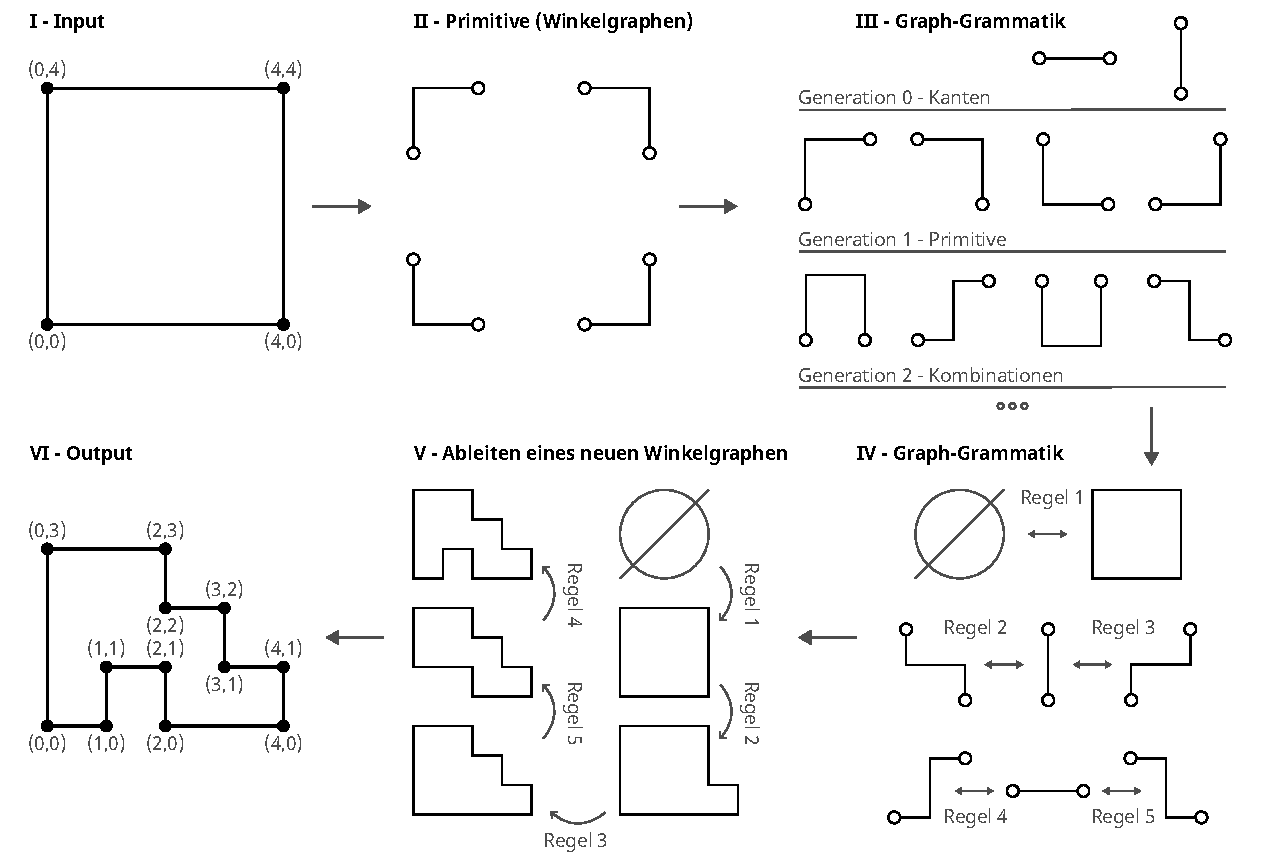
\includegraphics[height=\imgHeight]{images/overview.pdf}
    \caption{Zerteilen des Inputs und Aufbauen der Hierarchie}
    \label{fig:overview}
\end{figure}

Beim Aufbau der Hierarchie werden die neu entstehenden Graphen auf bestimmte
Eigenschaften überprüft, die es uns erlauben, daraus Regeln für ein Graphersetzungssystem abzuleiten. Das einfachste Beispiel hierfür sind
vollständige Graphen, also Graphen, die nur noch aus in sich geschlossenen Kreisen bestehen und keine Halbkanten mehr besitzen. Aus diesen lässt
sich eine sogennante Startregel ableiten, welche den leeren Graphen mit dem gefundenen vollständigen Graphen ersetzt. Das Finden von weiteren
Regeln ist deutlich komplizierter und wird später im Detail erläutert.

% TODO: Bild von Startregel

Sobald man nun eine Menge von Regeln für das Graphersetzungssystem gefunden hat, kann man diese verwenden um verschiedenste zum Inputgraphen
ähnliche Graphen abzuleiten, indem zufällig verschiedene Regeln nach und nach angewendet werden. Für einen solchen Graphen müssen dann noch
konkrete Knotenpositionen und Kantenlängen bestimmt werden, sodass dieser wieder als Struktur aus Polygonen dargestellt werden kann.

\section{Grundlagen}
\subsection{Input}
Der Algorithmus kann mit beliebigen polygonalen Strukturen als Input arbeiten. Dies können einfache Rechtecke oder aber auch komplizierte Gebilde
aus verschiedenen Häusern oder ähnlichem sein. Wichtig ist lediglich, dass der Input als Sammlung von Polygonen beschrieben werden kann, welche
wiederum als Sammlung von Punkten und Kanten beschrieben werden können.
So sind z.B. Kreise oder andere Strukturen mit Rundungen kein valider Input und können wenn dann nur durch komplexe Polygone angenähert werden.
Die einzelnen Polygone können außerdem mit Farben versehen werden, um verschiedene Arten von abgegrenzte Bereichen im Input zu markieren.

\subsection{Der Winkelgraph}
Zur Verarbeitung des Inputs wird dieser in einen sogenannten Winkelgraphen umgewandelt, in welchem die spezifischen Positionen der Knoten
keine Rolle spielen. Stattdessen wird nur abgebildet, welche Knoten es überhaupt gibt, welche der Knoten durch Kanten miteinander verbunden
sind, und in welchem Winkel diese Kanten verlaufen.
Die Kanten im Graphen werden mit einem entsprechenden Label versehen, welches neben den Start- und Endknoten ebenfalls Informationen zum
daraus ableitbaren Tangentenwinkel, sowie zu den Farben der links und rechts anliegenden Polygone enthält. Ein Kantenlabel besitzt die Form
\(\tilde{k} = (l,r,\theta)\), wobei \(\tilde{k}\) die Bezeichnung der Kante, \(l\) und \(r\) die Farben der anliegenden Polygone, und
\(\theta\) der Tangentenwinkel der Kante sind.
Nach der Umwandlung des Inputs in einen Winkelgraphen ist dieser zunächst \textit{vollständig}, d.h. er besteht ausschließlich aus
geschlossenen Kreisen. In späteren Verarbeitungsschritten wird dieser allerdings in unvollständige Teilgraphen zerlegt, welche dann außerdem
\textit{Halbkanten} enthalten können. Im Gegensatz zu den vorher erwähnten Kanten sind diese gerichtet, können aber trotzdem durch ein
gleichartiges Kantenlabel beschrieben werden. In späteren Abschnitten wird noch etwas genauer auf die Relevanz von Halbkanten und deren
spezifische Notation eingegangen.

\subsection{Lokale Ähnlichkeit}
Ziel des Algorithmus ist es, Variationen des Inputs zu erzeugen. Dabei soll der Output eine gewisse Ähnlichkeit zum Input beibehalten. Global
vorzugehen und die vollständigen Input- und Output-Strukturen miteinander zu vergleichen führt hierbei allerdings zu keinem vernünftigen
Ergebnis. Der Output muss sich zumindest teilweise vom Input unterscheiden, ansonsten ist das Ergebnis nicht zu gebrauchen. Um Vergleiche
auf einer kleineren Ebene vornehmen zu können, stellen wir hier das Konzept der \textit{lokalen Ähnlichkeit} vor.

% TODO: Formulierung verbessern
Zwei Polygonstrukturen sind sich lokal ähnlich, wenn sich jeder Teil der einen Struktur zu einem Teil der anderen Struktur zuordnen lässt. Es
müssen sich also alle Kanten und Polygonfarben mit gleicher Anordnung irgendwo in beiden Strukturen finden lassen. Befindet sich im Input z.B.
ein Eckpunkt, welcher mit einer vertikalen und einer horizontalen Kante verbunden ist, so muss der Output ebenfalls einen Eckpunkt enthalten,
der an einer vertikalen und einer horizontalen Kante anliegt.

% TODO: Beispielbild
\begin{figure}[h]
    \centering
    
\includegraphics[height=\imgHeight]{images/referencegrid.pdf}
    \caption{reference grid}
    \label{fig:reference}
\end{figure}

Ein verwandtes Konzept, das zum Verständnis beitragen kann, ist das der \textit{r-Ähnlichkeit} \cite{3_bokeloh_et_al}. Zwei Strukturen sind hier
\textit{r}-ähnlich, wenn wir für jeden Punkt innerhalb der einen Struktur einen Kreis mit Radius \textit{r} aufspannen können und sich der Inhalt
dieses Kreises (r-Nachbarschaft des Punktes) genauso in der anderen Struktur wiederfinden lässt.

% TODO: Beispielbild
\begin{figure}[h]
    \centering
    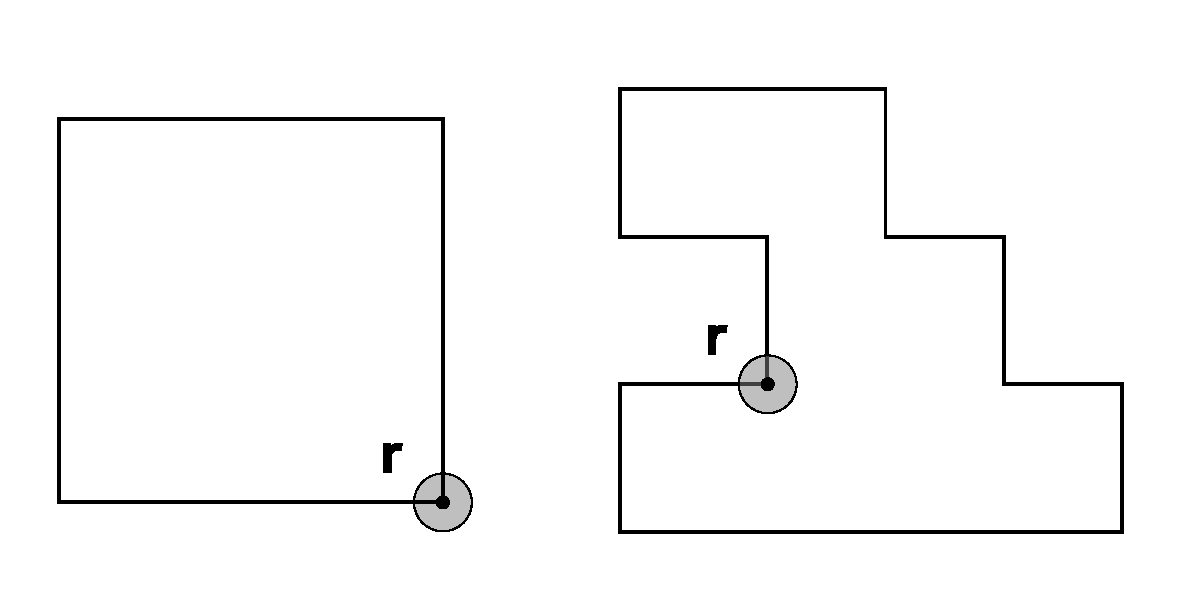
\includegraphics[height=\imgHeight]{images/test.pdf}
    \caption{Beispiel für r-Ähnlichkeit}
\end{figure}

Die hier verwendete lokale Ähnlichkeit funktioniert nach dem gleichen Konzept, mit der Ausnahme, dass der Radius so klein wie möglich gehalten
wird. Wir schauen uns also lediglich an, welche Kanten und Polygone direkt an einem Punkt anliegen, während uns die restliche Nachbarschaft
egal ist. So können die betrachteten Strukturen beliebig skaliert werden und trotzdem ihre lokale Ähnlichkeit zueinander bewahren, solang alle
Kantenwinkel dabei beibehalten werden.

\subsection{Planarität und der Graph Boundary String}
% inkl. Erklärung zu Turns

% TODO: was genau hat Boundary String mit der Planarität zu tun?

\subsection{Grundlegende Operationen}
\textit{Teil-Operation.}
Eine Kante \(\tilde{k}\) kann in zwei Halbkanten \(k\) und \(\overline{k}\) zerteilt werden. Im Gegensatz zu \(\tilde{k}\)
sind diese beiden Halbkanten gerichtet und zeigen in entgegengesetze Richtungen. Dabei zeigt k stets in positive Richtung und besitzt einen
positiven Tangentenwinkel \(\theta \in [0\degree,180\degree) \), während \(\overline{k}\) immer in negative Richtung zeigt und einen negativen
Tangentenwinkel \(\theta \in [-180\degree,0\degree) \) besitzt. Ein Tangentenwinkel von 0° zählt hier als positiv. Der entgegengesetze Winkel
von 180\degree\ gilt als negativ, da dieser ebenfalls als -180\degree\ interpretiert werden kann. Die Teil-Operation ermöglicht das Zerlegen vom
Input in die jeweiligen Primitive.

\textit{Klebe-Operation.}
Zwei entgegengesetze Halbkanten \(k\) und \(\overline{k}\) können wieder zu einer vollständigen und ungerichteten Kante
\(\tilde{k}\) zusammengeklebt werden. Dies ermöglicht die Kombination von mehreren kleineren Graphen, vorausgesetzt diese besitzen passende
Halbkanten. Die Klebe-Operation stellt somit das Gegenteil zur Teil-Operation dar und wird dazu genutzt, Schritt für Schritt die Graph-Hierarchie
aufzubauen.

% TODO: Branch und Loop Gluing erklären?

\section{Ablauf}
\subsection{Anpassen des Inputs}
Bevor wir mit dem Verfahren beginnen können, muss der Input an bestimmte Anforderungen angepasst werden. Die übergebene Polygonstruktur
kann so nicht direkt verarbeitet werden und muss erst einmal in einen Winkelgraphen umgewandelt werden. Dazu werden zunächst einfach
alle Knoten und
Kanten aus dem Input übernommen. Anschließend werden die Knotenpositionen genutzt, um den Verlauf der Kanten in Form eines Tangentenwinkels zu
ermitteln. Sobald dies geschehen ist, können die Knotenpositionen dann ignoriert werden, da lediglich die Ausrichtung der Kanten eine Rolle
für die weiteren Schritte spielt. Die restlichen Informationen zur Geometrie werden nicht benötigt und erst beim Erzeugen des finalen Outputs
wieder festgelegt.

\subsection{Finden der Primitive}
Ist nun der Winkelgraph ermittelt worden, können wir daraus die Primitive ableiten. Diese sind die fundamentalen Grundbausteine für das
gesamte Verfahren. Aus ihnen werden alle weiteren Strukturen abgeleitet, weshalb es besonders wichtig ist, diese korrekt und vollständig zu
ermitteln. Glücklicherweise wird dies durch die vorgestellte Teil-Operation recht trivial. Wenden wir diese auf jede Kante des gegebenen
Winkelgraphen an, so bleiben nur Teilgraphen übrig, welche nur aus einem einzelnen Knoten, sowie einigen Halbkanten bestehen. Diese Teilgraphen
sind dann auch schon die gesuchten Primitive. Hier können allerdings einige identische Teilgraphen entstehen, falls Teile des Input eine ähnliche
Struktur vorzuweisen hatten. Solche Duplikate sollen natürlich nicht in die weiteren Schritte des Verfahrens übernommen werden und müssen daher
entfernt werden.

\subsection{Aufbauen der Hierarchie}

